\documentclass{article}
\usepackage[letterpaper, margin=1in]{geometry}
\usepackage{amsmath}
\usepackage{amsfonts}
\usepackage{amssymb}
\usepackage{graphicx}
\usepackage{hyperref}
\graphicspath{ {./graphs/} }

\title{US-Mexico Border Apprehensions Sweave Report} 
\author{Michael Rojas, Kerin Grewal}

\usepackage{Sweave}
\begin{document}
\maketitle
\Sconcordance{concordance:Shiny_App_Sweave.tex:Shiny_App_Sweave.Rnw:%
1 59 1 1 2 1 0 1 2 14 0 2 2 1 1 29 0 1 3 241 1 1 2 1 0 1 1 2 2 1 3 14 0 %
1 2 14 0 1 2 1 1 25 0 1 2 1 1 26 0 1 2 1 1}


\pagebreak

\section{CNN report Summary}

\begin{center}

US-Mexico boarder apprehensions have been steadily declining since 2000, and in April of 2017 they reached historic lows. These downward trends and record lows can be accredited to President Trump’s election. The data shows that President Trump’s aggression towards immigration laws is having a deterring effect, and migrants are less enticed to enter the country. DHS credits the administration policy as the lowest apprehensions prior to this past April were in December of 2011. This new low is 7,000 apprehensions less than the previous. In a year since April 2016, apprehensions were down 62%, though there are multiple different reasons for such a change.
Here you can find the monthly summaries of apprehensions by sector in a time series from 2000 to 2017 depicting the changes throughout time.\\
.\\

Below is a link to the original story and Video that is linked to these Apprehensions\\

\end{center}
\url{https://www.cnn.com/2017/05/09/politics/border-crossings-apprehensions-down-trump/index.html}\\

\begin{center}
The following graph represents a Summary of the Apprehensions made at the US-Mexico border between the years 2000 through the year 2017. Each green marker represents the average apprehension rate for that year.\\
.\\

\end{center}


\subsection{Figure 1}

\begin{figure}[h]
\centering
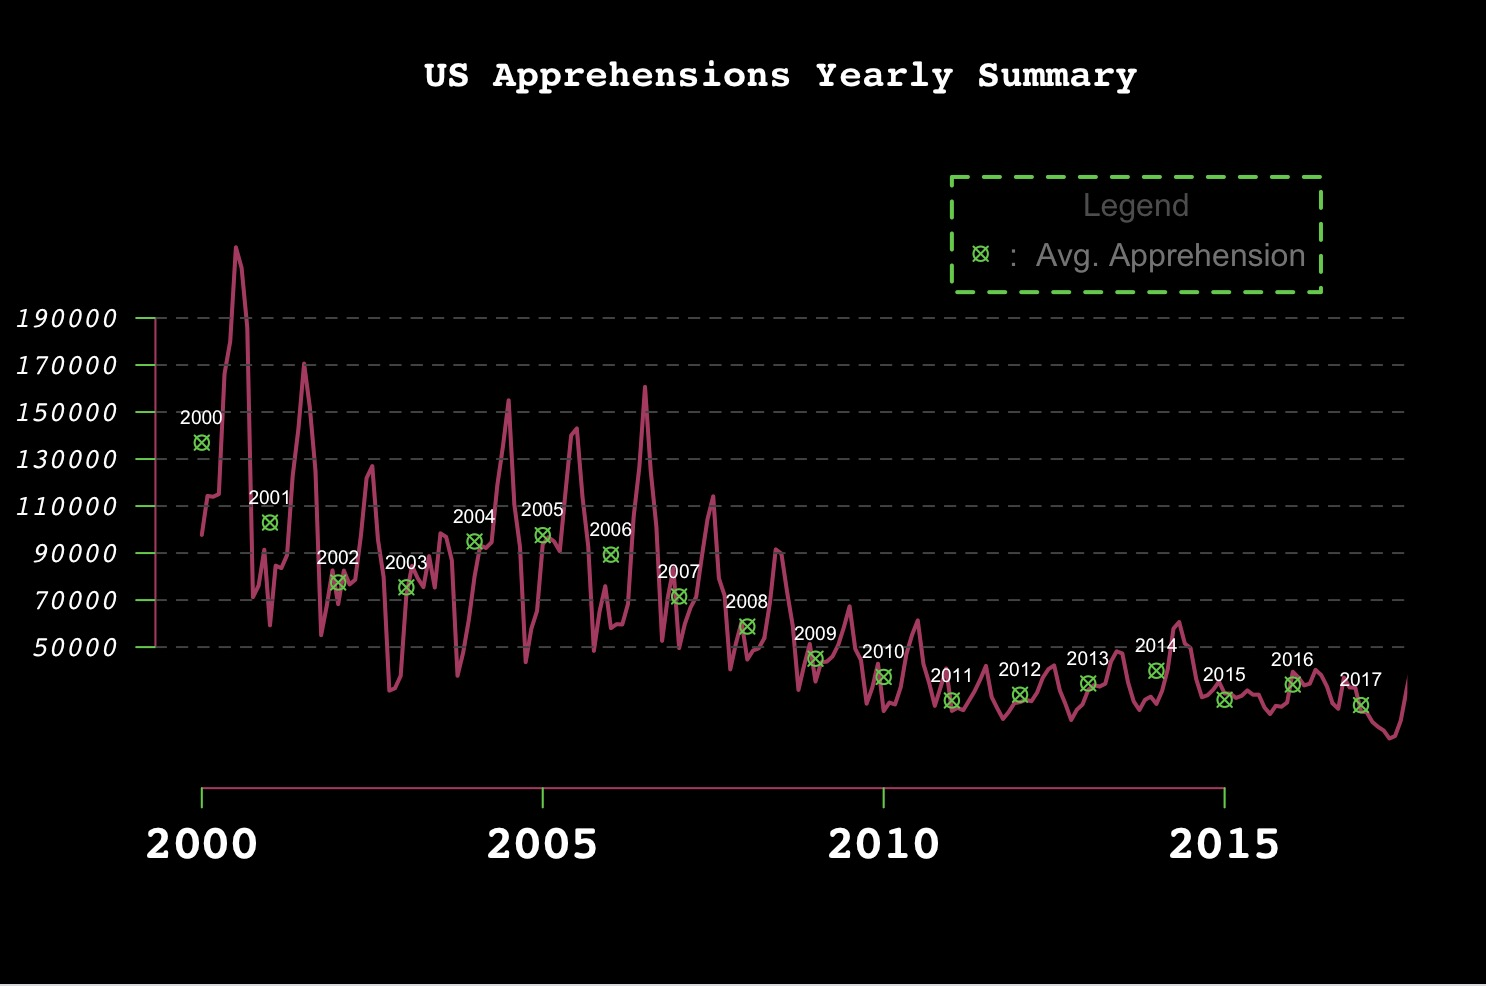
\includegraphics[ height=9cm, width=16cm]{SummaryPlot}
\caption{Us Apprehension Summary Plot}
\end{figure}


.\\
.\\
It is seen from the figure above that Apprehensions throughout time have been slowly decreasing, and it is now as low as it once was back in the year 2011. This is being accredited to Donald Trumps aggression on border patrol and the desire to build a higher wall to prevent the US from having Mexicans or anybody fleeing their country to illegally cross the border into the states

\pagebreak

\subsection{Statistical Tests}
\begin{center}
Below are some statistical tests on the data on the boarder apprehensions from 2000 to 2017.\\
.\\

\end{center}
\begin{Schunk}
\begin{Sinput}
> summ <- read.csv('PB monthly summaries.csv')
> t.test(summ)
\end{Sinput}
\begin{Soutput}
	One Sample t-test

data:  summ
t = 21.149, df = 233, p-value < 2.2e-16
alternative hypothesis: true mean is not equal to 0
95 percent confidence interval:
 51572.25 62168.34
sample estimates:
mean of x 
  56870.3 
\end{Soutput}
\begin{Sinput}
> qqnorm(summ[,7])
> summ$year=NULL
> summary(summ)
\end{Sinput}
\begin{Soutput}
    October         November        December        January      
 Min.   :25612   Min.   :22405   Min.   :18983   Min.   : 21514  
 1st Qu.:33371   1st Qu.:32048   1st Qu.:25262   1st Qu.: 27358  
 Median :44561   Median :37524   Median :34408   Median : 51765  
 Mean   :50876   Mean   :43752   Mean   :36674   Mean   : 64269  
 3rd Qu.:64491   3rd Qu.:56319   3rd Qu.:43523   3rd Qu.: 91122  
 Max.   :91410   Max.   :76196   Max.   :71252   Max.   :185979  
    February          March            April             May        
 Min.   : 18754   Min.   : 12195   Min.   : 11127   Min.   : 14519  
 1st Qu.: 32445   1st Qu.: 43487   1st Qu.: 42524   1st Qu.: 41217  
 Median : 61347   Median : 78556   Median : 66926   Median : 64958  
 Mean   : 75078   Mean   : 92433   Mean   : 82641   Mean   : 73899  
 3rd Qu.:107219   3rd Qu.:139034   3rd Qu.:125384   3rd Qu.:103444  
 Max.   :211328   Max.   :220063   Max.   :180050   Max.   :166296  
      June             July            August         September    
 Min.   : 16087   Min.   : 18187   Min.   : 22288   Min.   :22537  
 1st Qu.: 33325   1st Qu.: 29598   1st Qu.: 30526   1st Qu.:27515  
 Median : 55858   Median : 46658   Median : 46032   Median :42104  
 Mean   : 58129   Mean   : 55020   Mean   : 55583   Mean   :48953  
 3rd Qu.: 77874   3rd Qu.: 78628   3rd Qu.: 84004   3rd Qu.:66016  
 Max.   :115093   Max.   :113956   Max.   :114312   Max.   :97744  
\end{Soutput}
\begin{Sinput}
> 
\end{Sinput}
\end{Schunk}

\pagebreak
\section{Top three Month Periods with the most Apprehensions}
.\\
Looking at the data and being able to manipulate and run a quick analysis on the apprehensions for both 2010 and 2017 we came up with the following conclusions for the most apprehensions in those years respectively by using the following scrypt:\\

\begin{figure}[h]
\centering
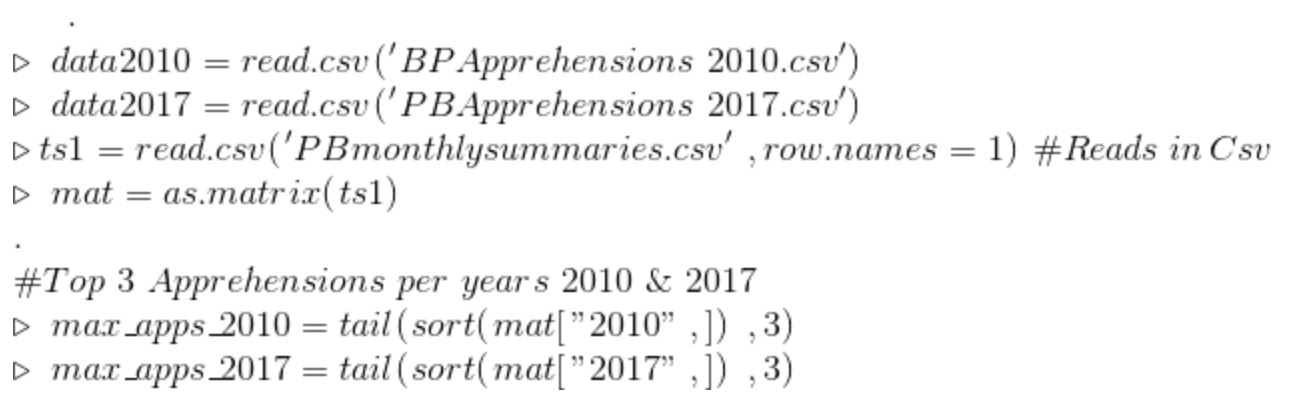
\includegraphics{code}
\caption{Code Executed To find Max Apprehensions}
\end{figure}

.\
The following is the output of the code executed above:\\

\begin{figure}[h]
\centering
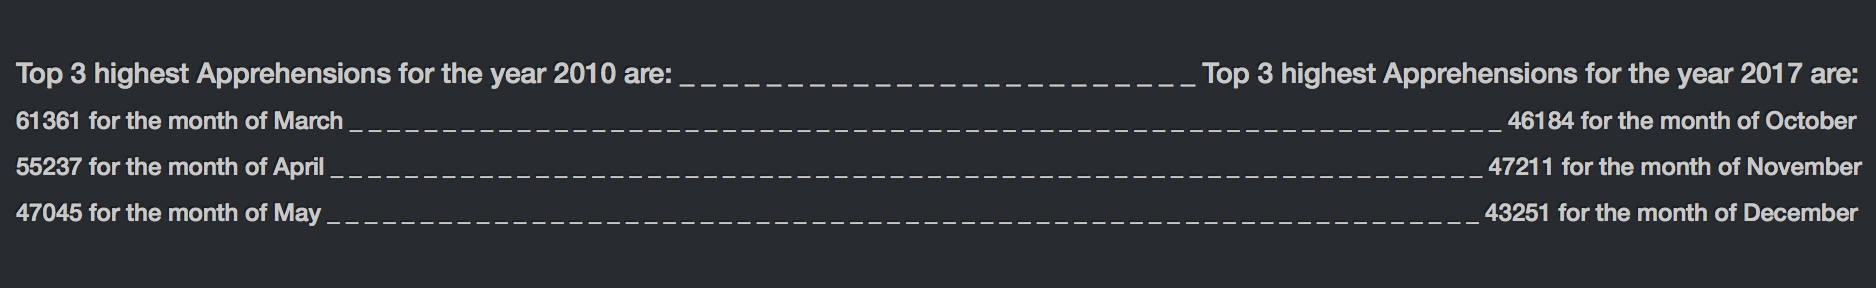
\includegraphics[ height=3cm, width=18cm]{Top3}
\caption{Max Apprehensions For the Years 2010 and 2017}
\end{figure}

\section{Change in Maximum}

Using simple statistical tests like those demonstrated in class we were able to compare the sector with the most apprehensions for 2010 and with the sector with the most apprehensions in 2017. Depicted in the graph above It is noted that the maximum apprehensions for the year 2010 was 61361 for the month of March and the maximum apprehensions for the year 2017 was 47211 for the month of November. The difference in Apprehensions was a total of 14150 people that were being detained or sent back home.

\pagebreak

\section{Data Visualizations}

Using R's built-in plotting methods, we are able to visualize US-Mexico Apprehension data, camparing the 2010 and 2017 statistics by month and sector. By using simple statistical tests like those demonstrated in class we are able to demonstrate side by side visualizations of the years 2010 and 2017 comparing the data by sector.\\


In the following plots you will be able to visualize the differences in years According to sector Beggining with:\\


\subsection{Big Bend}

\begin{figure}[h]
\centering
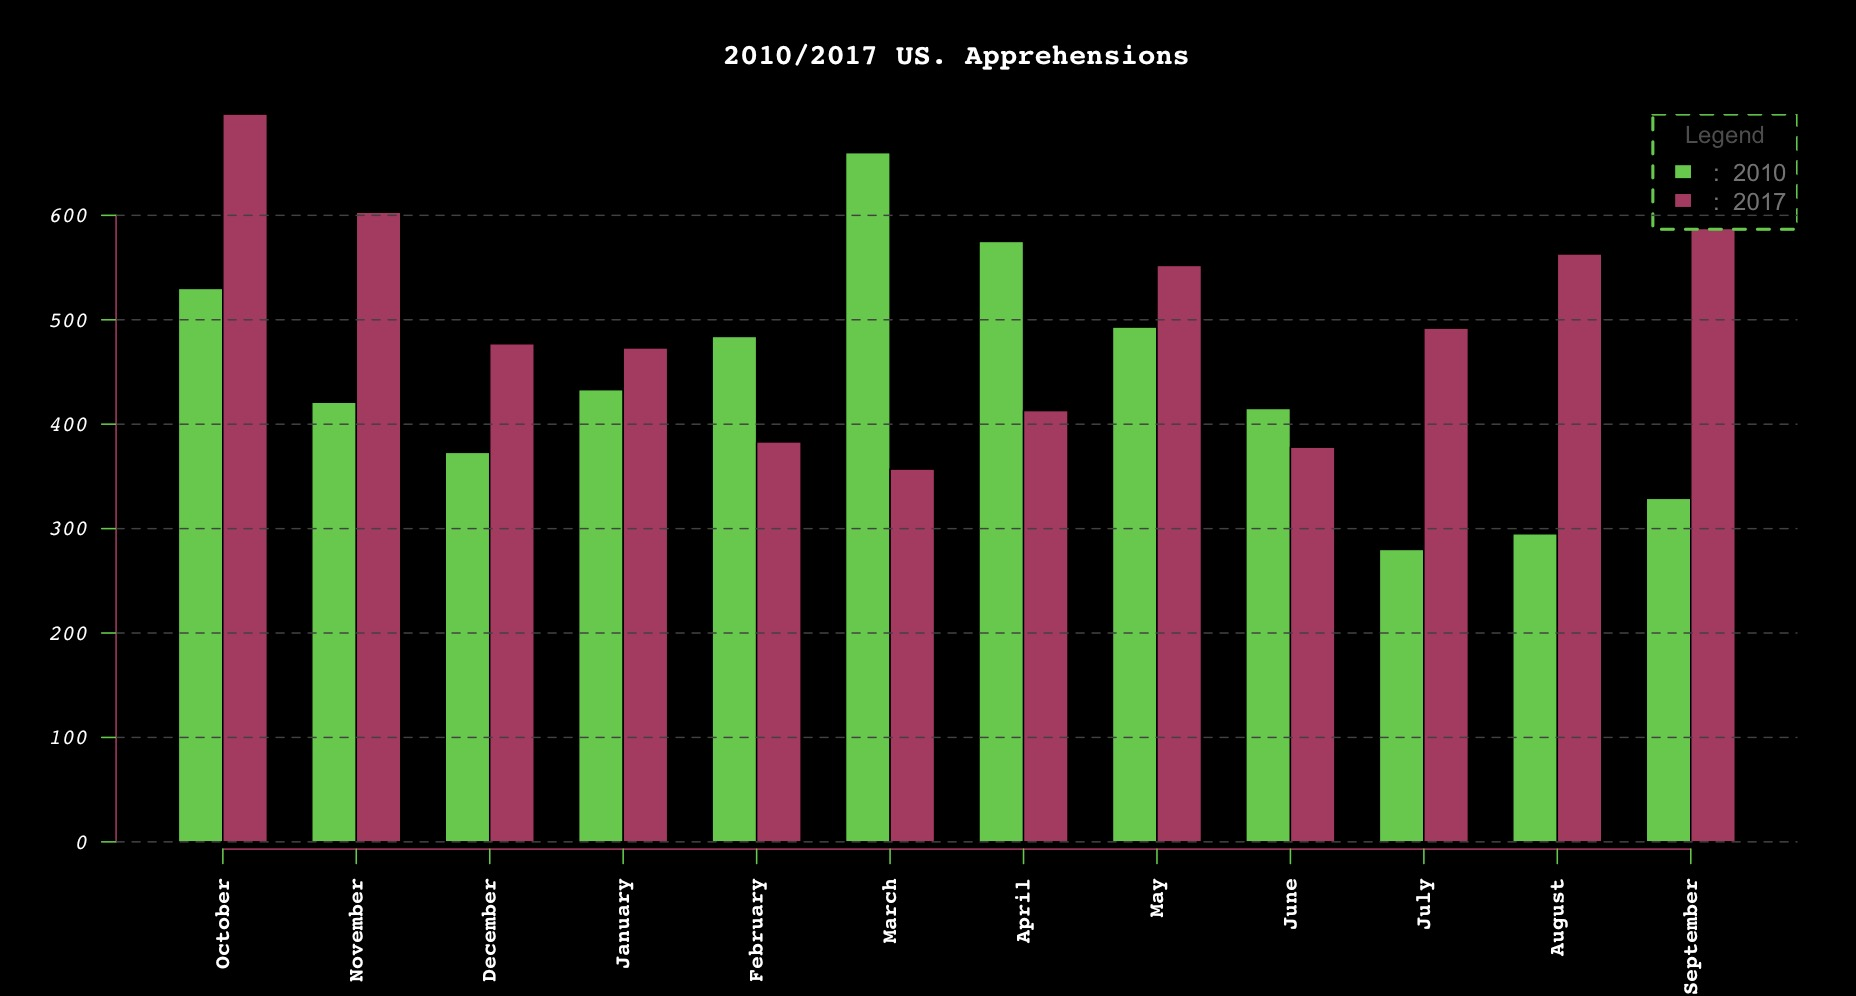
\includegraphics[ height=9cm, width=16cm]{BigBend}
\caption{Sector: Big Bend Apprehensions Plot}
\end{figure}
.\\

\begin{figure}[h]
\centering
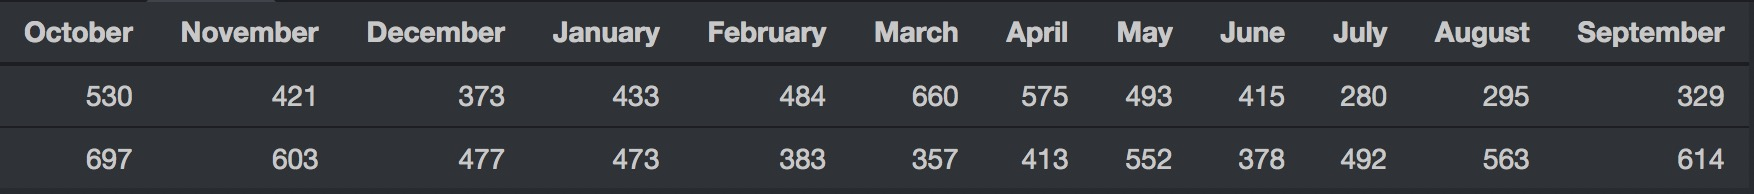
\includegraphics{BigBendTable}
\caption{Sector: Big Bend Apprehensions Table}
\end{figure}

\pagebreak

\subsection{Del Rio}

\begin{figure}[h]
\centering
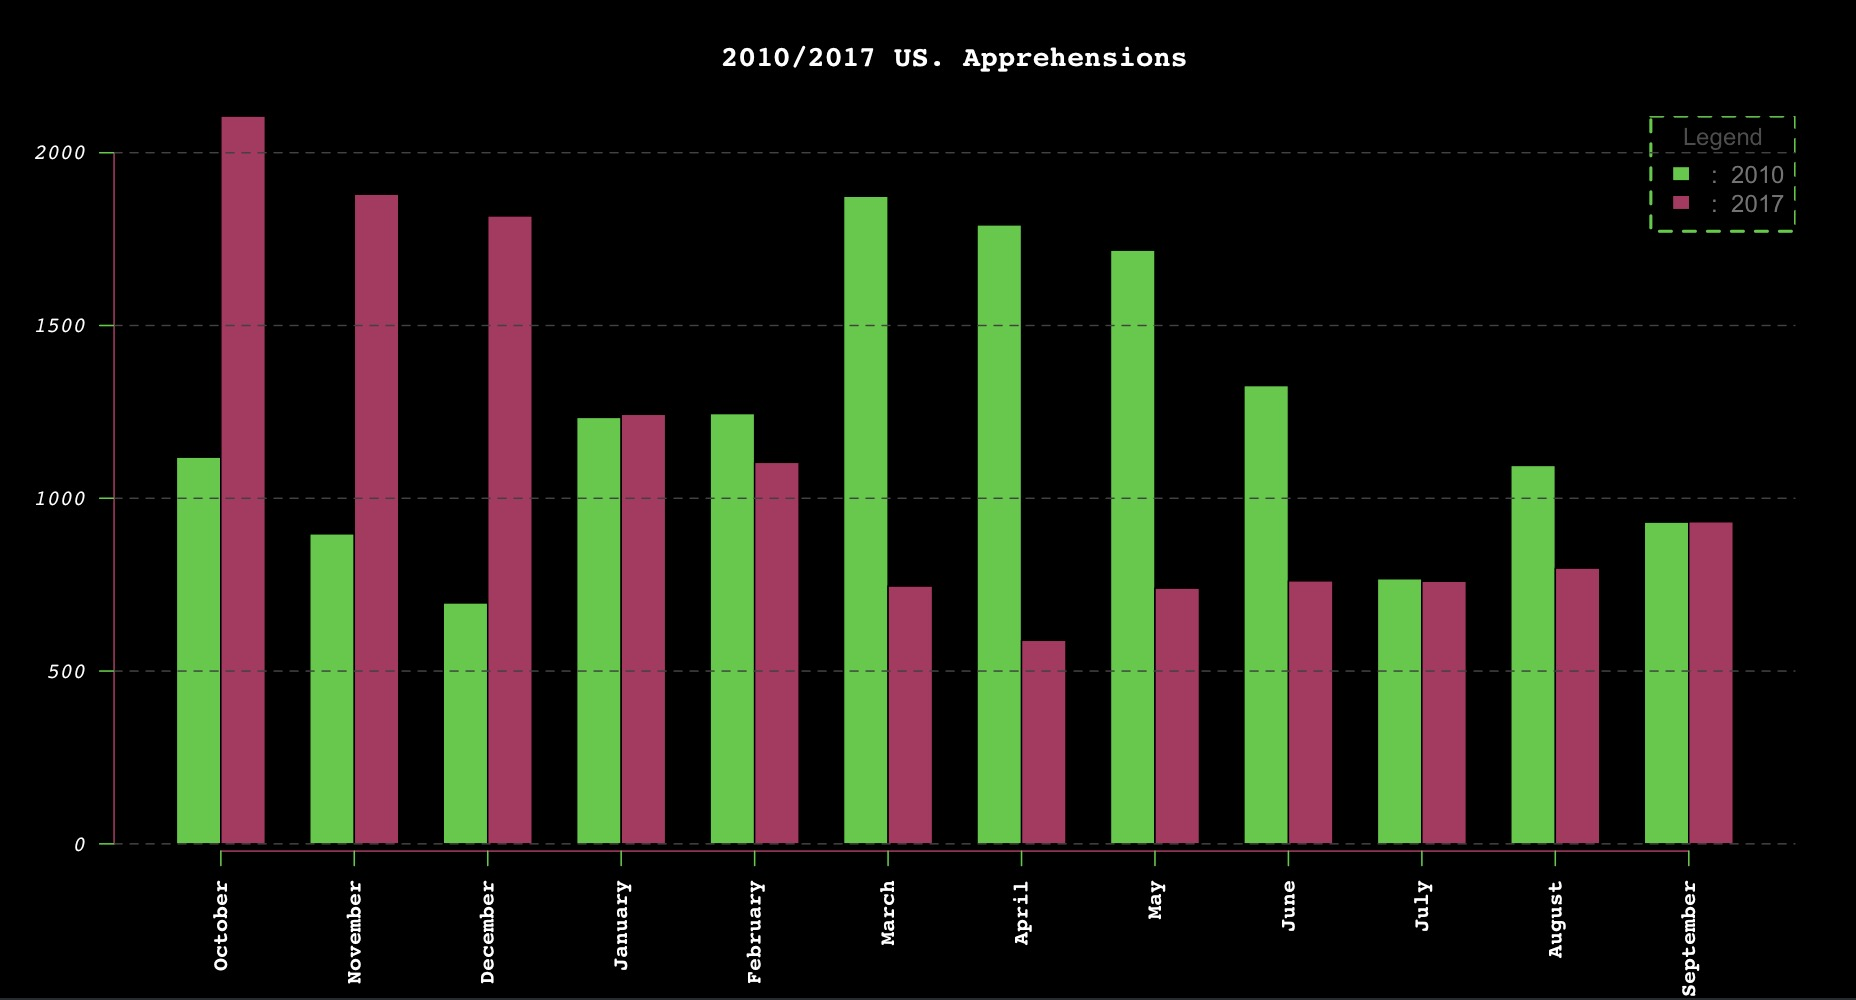
\includegraphics[ height=8cm, width=16cm]{DelRio}
\caption{Sector: Del Rio Apprehensions Plot}
\end{figure}
.\\

\begin{figure}[h]
\centering
\includegraphics[ height=4cm, width=11cm]{dRiopic}
\caption{Del Rio}
\end{figure}

\begin{figure}[h]
\centering
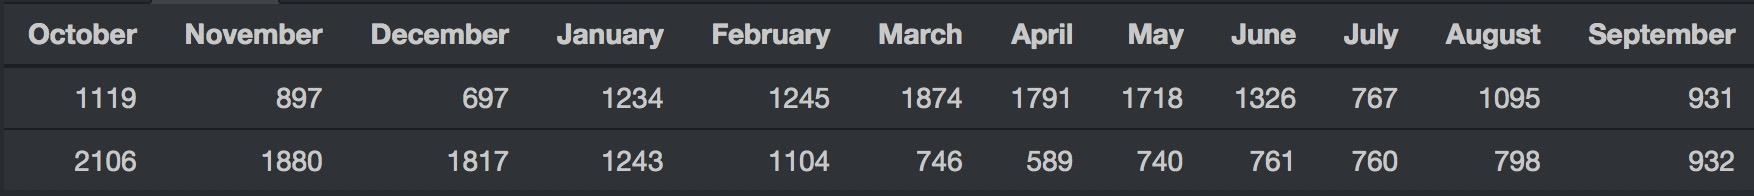
\includegraphics{DelRioTable}
\caption{Sector: Del Rio Apprehensions Table}
\end{figure}

\pagebreak

\subsection{El Centro}

\begin{figure}[h]
\centering
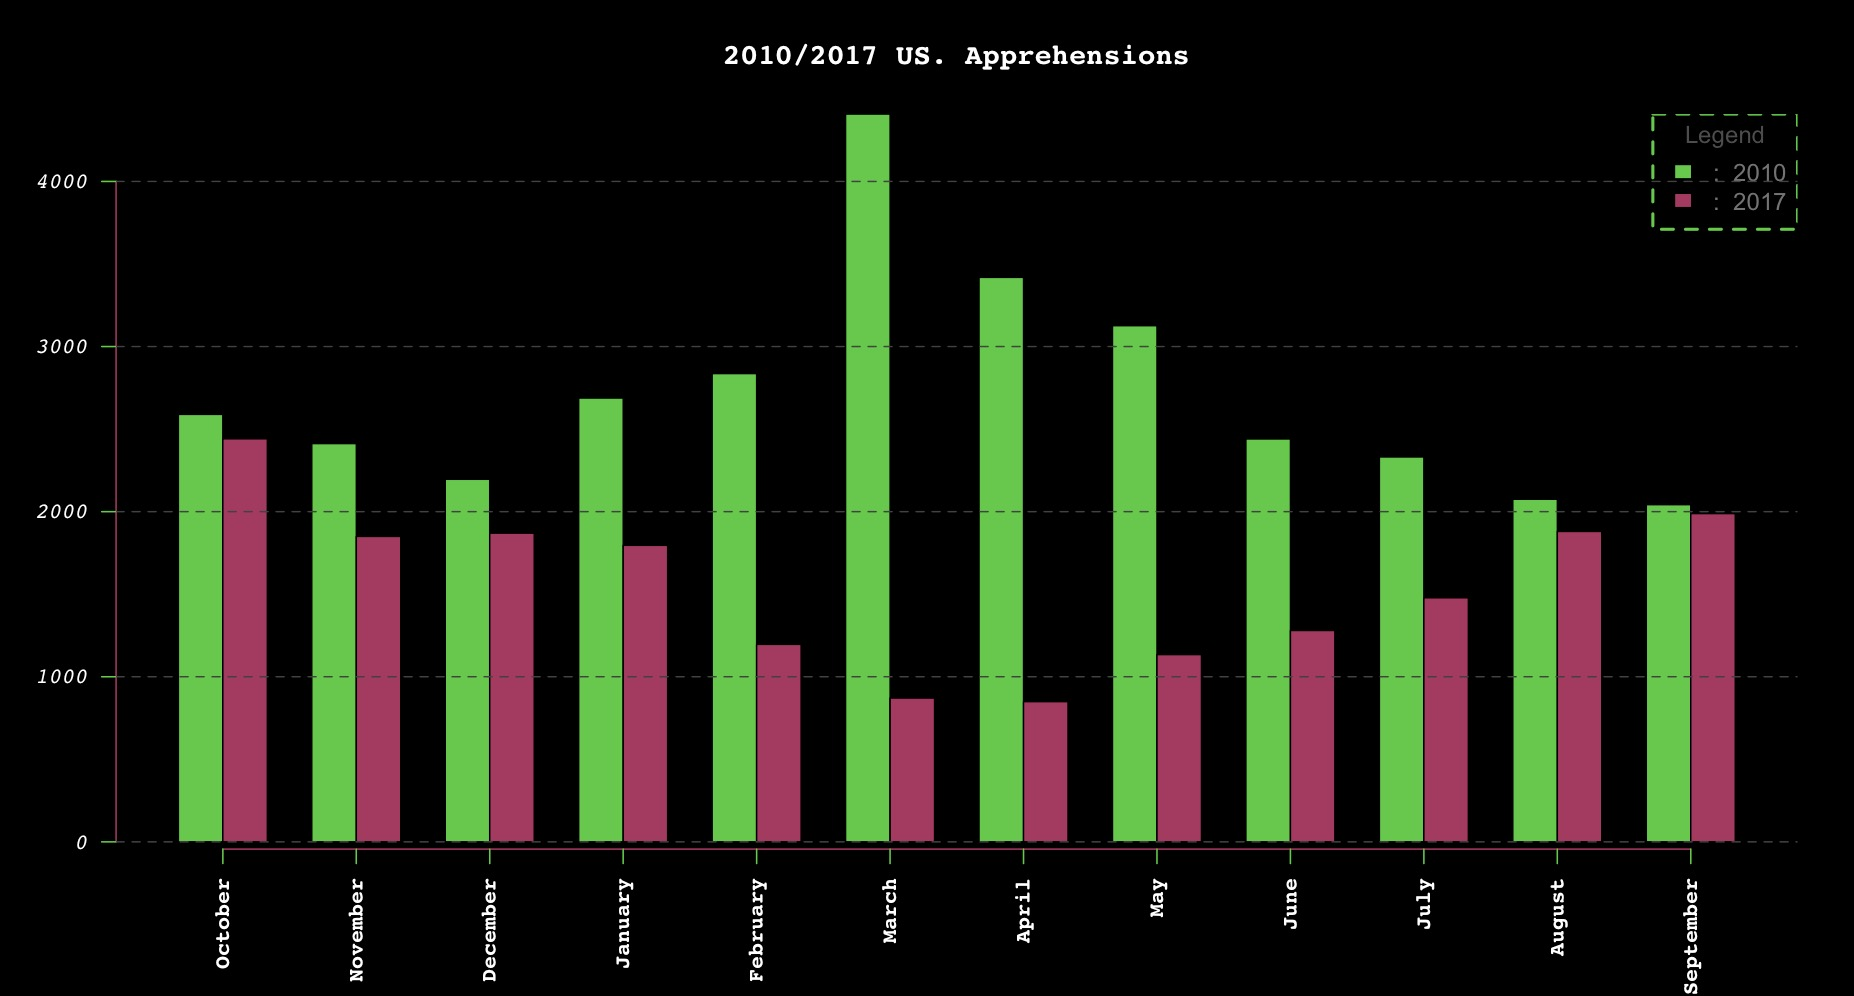
\includegraphics[ height=8cm, width=16cm]{ElCentro}
\caption{Sector: El Centro Apprehensions Plot}
\end{figure}
.\\

\begin{figure}[h]
\centering
\includegraphics[ height=4cm, width=11cm]{ElCentropic}
\caption{El Centro}
\end{figure}

\begin{figure}[h]
\centering
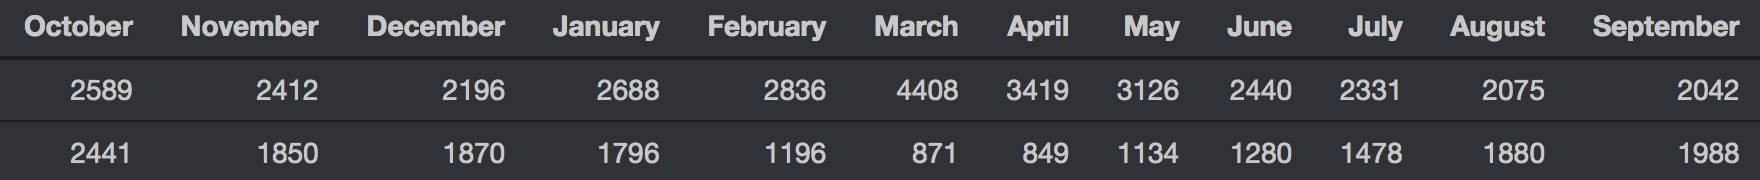
\includegraphics{ElCentroTable}
\caption{Sector: El Centro Apprehensions Table}
\end{figure}

\pagebreak

\subsection{El Paso}

\begin{figure}[h]
\centering
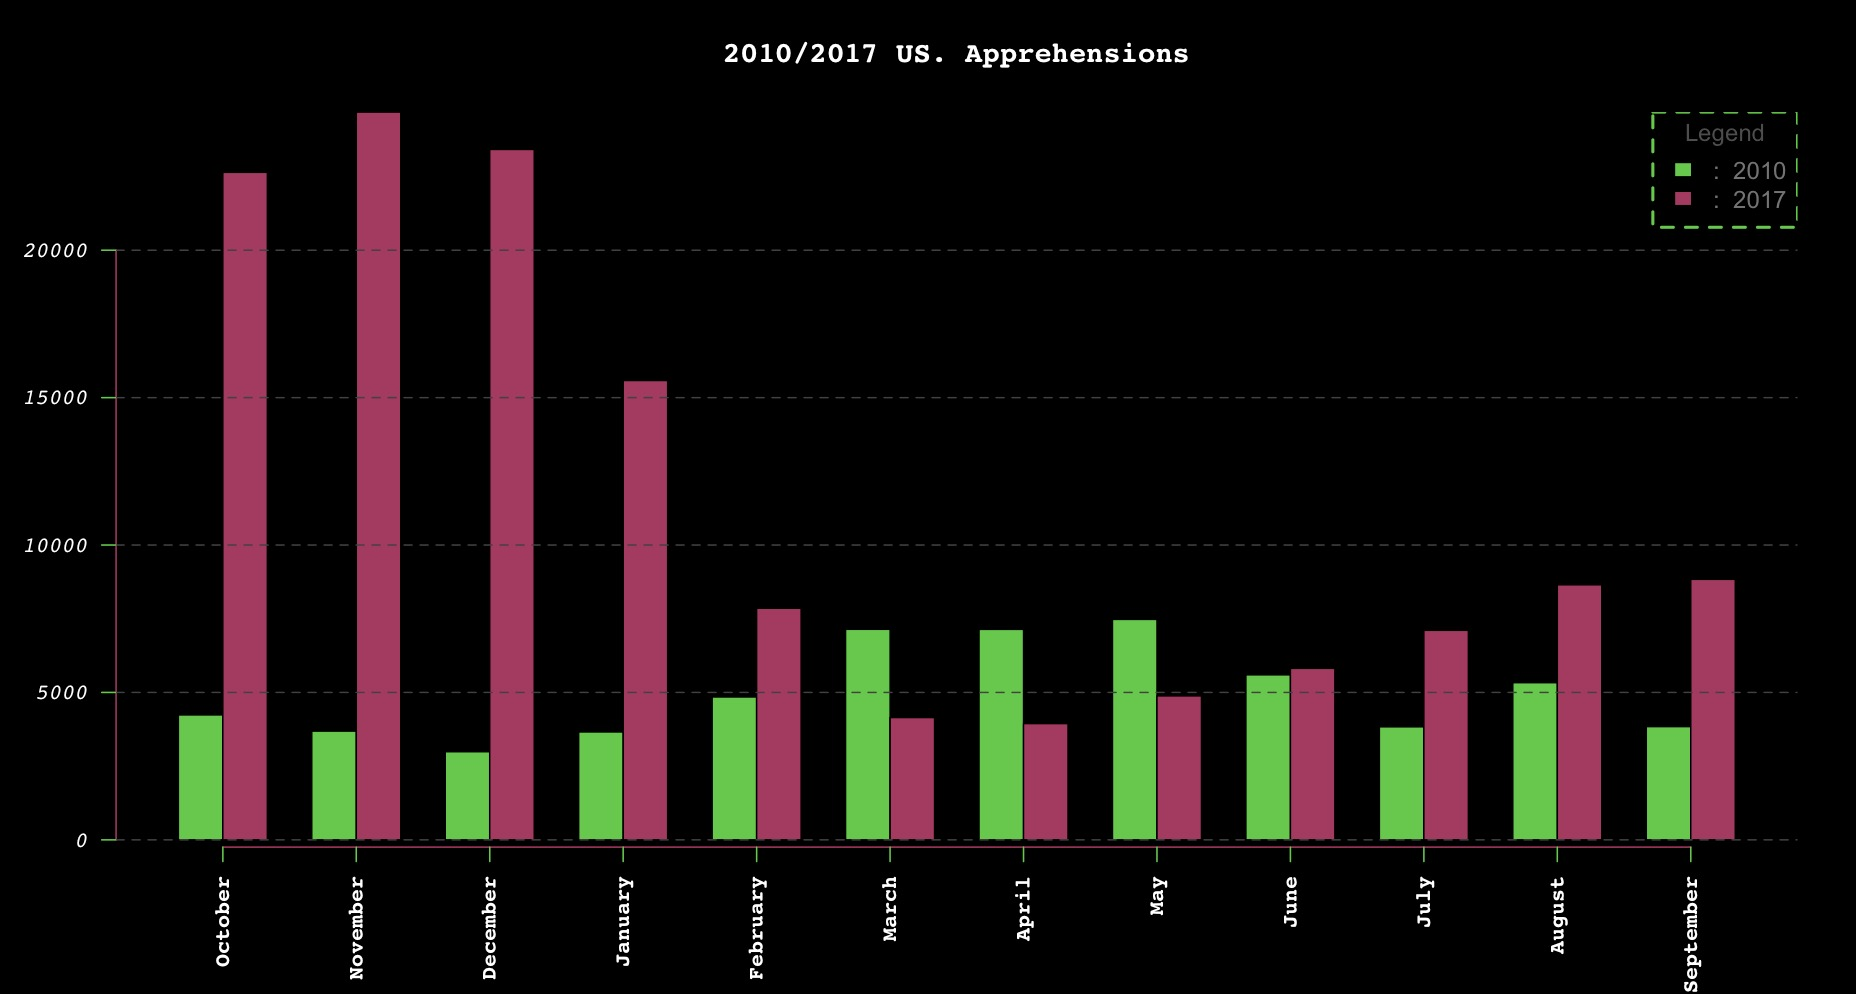
\includegraphics[ height=8cm, width=16cm]{ElPaso}
\caption{Sector: El Paso Apprehensions Plot}
\end{figure}
.\\

\begin{figure}[h]
\centering
\includegraphics[ height=4cm, width=11cm]{ElPasopic}
\caption{El Paso}
\end{figure}

\begin{figure}[h]
\centering
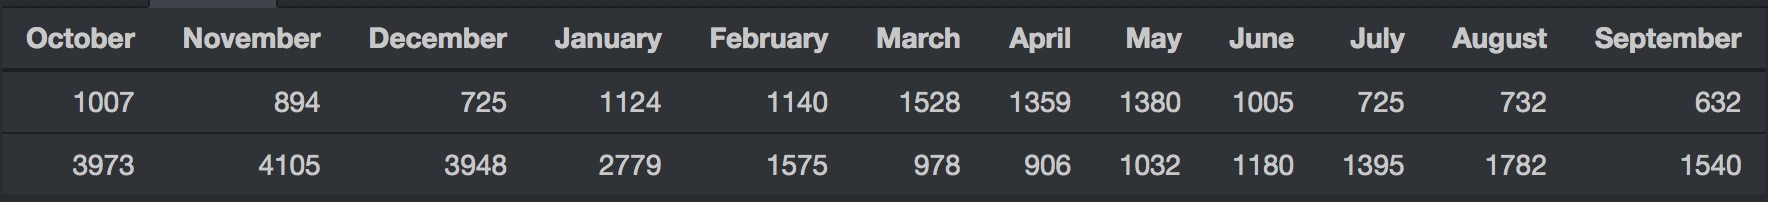
\includegraphics{ElPasoTable}
\caption{Sector: El Paso Apprehensions Table}
\end{figure}

\pagebreak

\subsection{Laredo}

\begin{figure}[h]
\centering
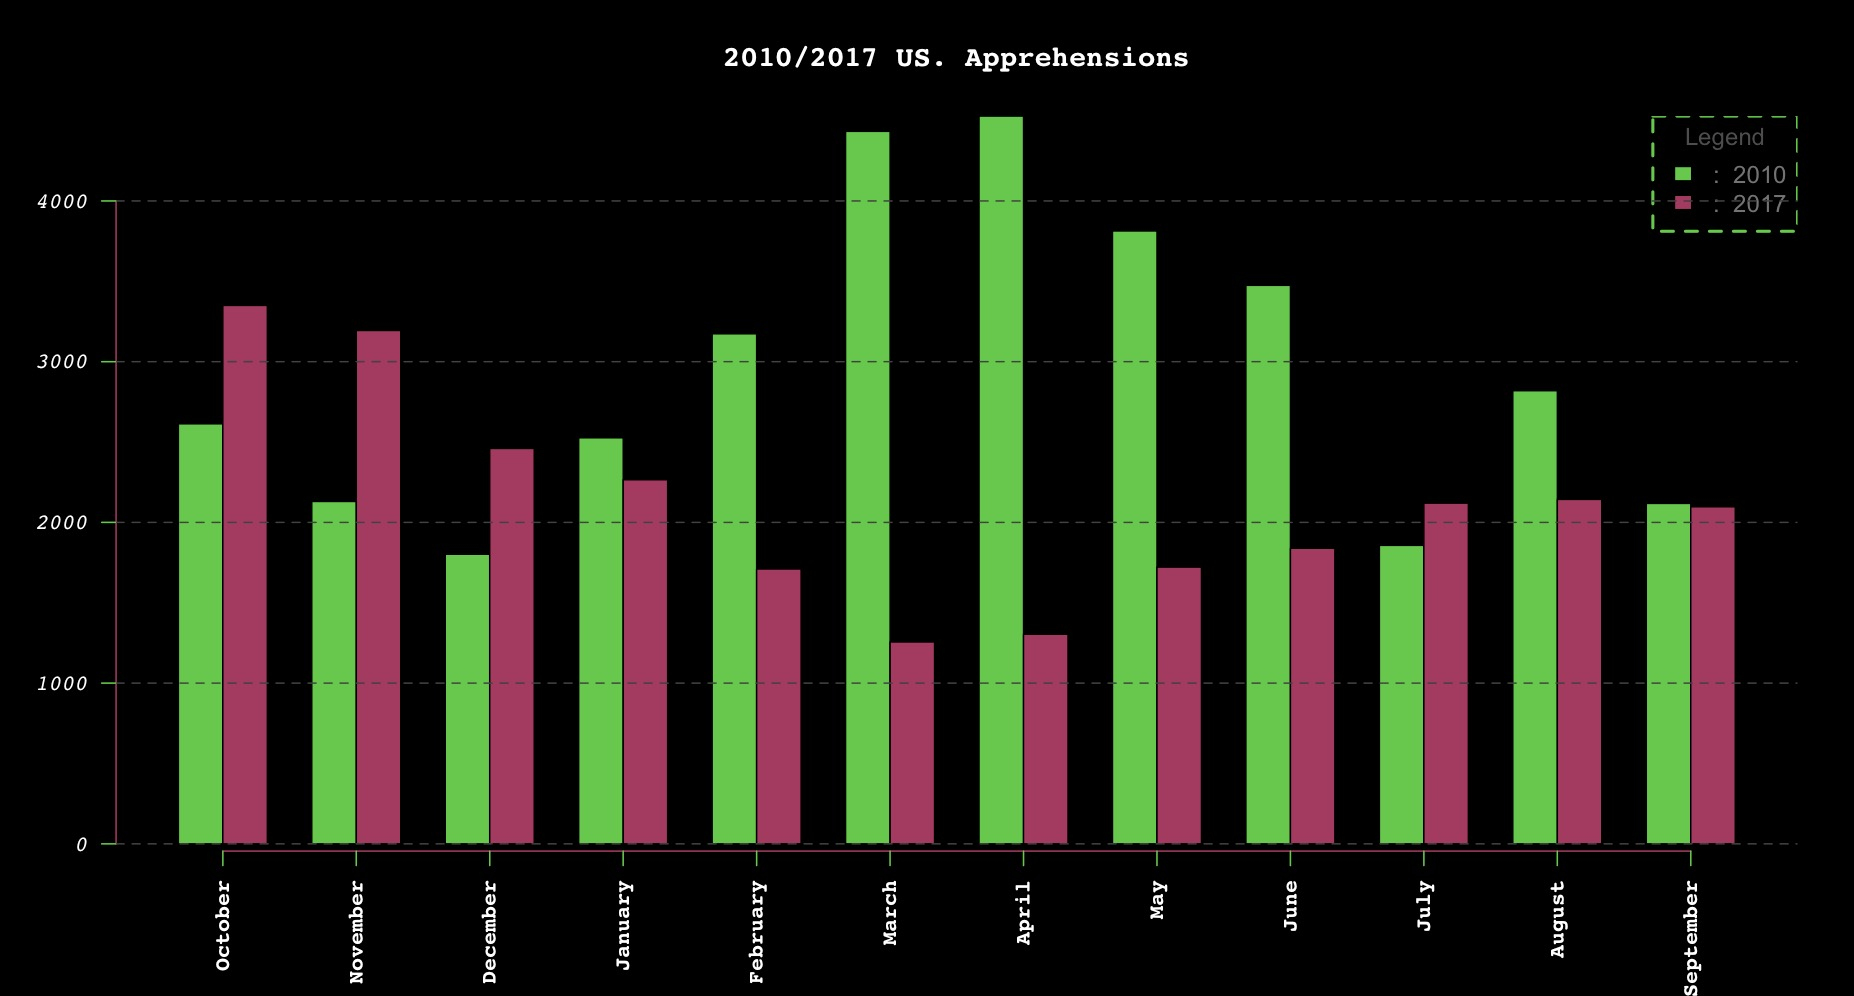
\includegraphics[ height=8cm, width=16cm]{Laredo}
\caption{Sector: Laredo Apprehensions Plot}
\end{figure}
.\\

\begin{figure}[h]
\centering
\includegraphics[ height=4cm, width=11cm]{Laredopic}
\caption{Laredo}
\end{figure}

\begin{figure}[h]
\centering
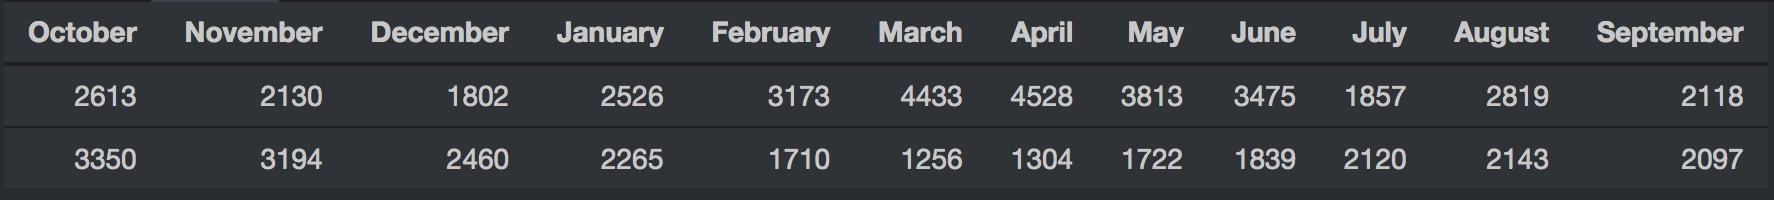
\includegraphics{LaredoTable}
\caption{Sector: Laredo Apprehensions Table}
\end{figure}

\pagebreak

\subsection{Rio Grande Valley}

\begin{figure}[h]
\centering
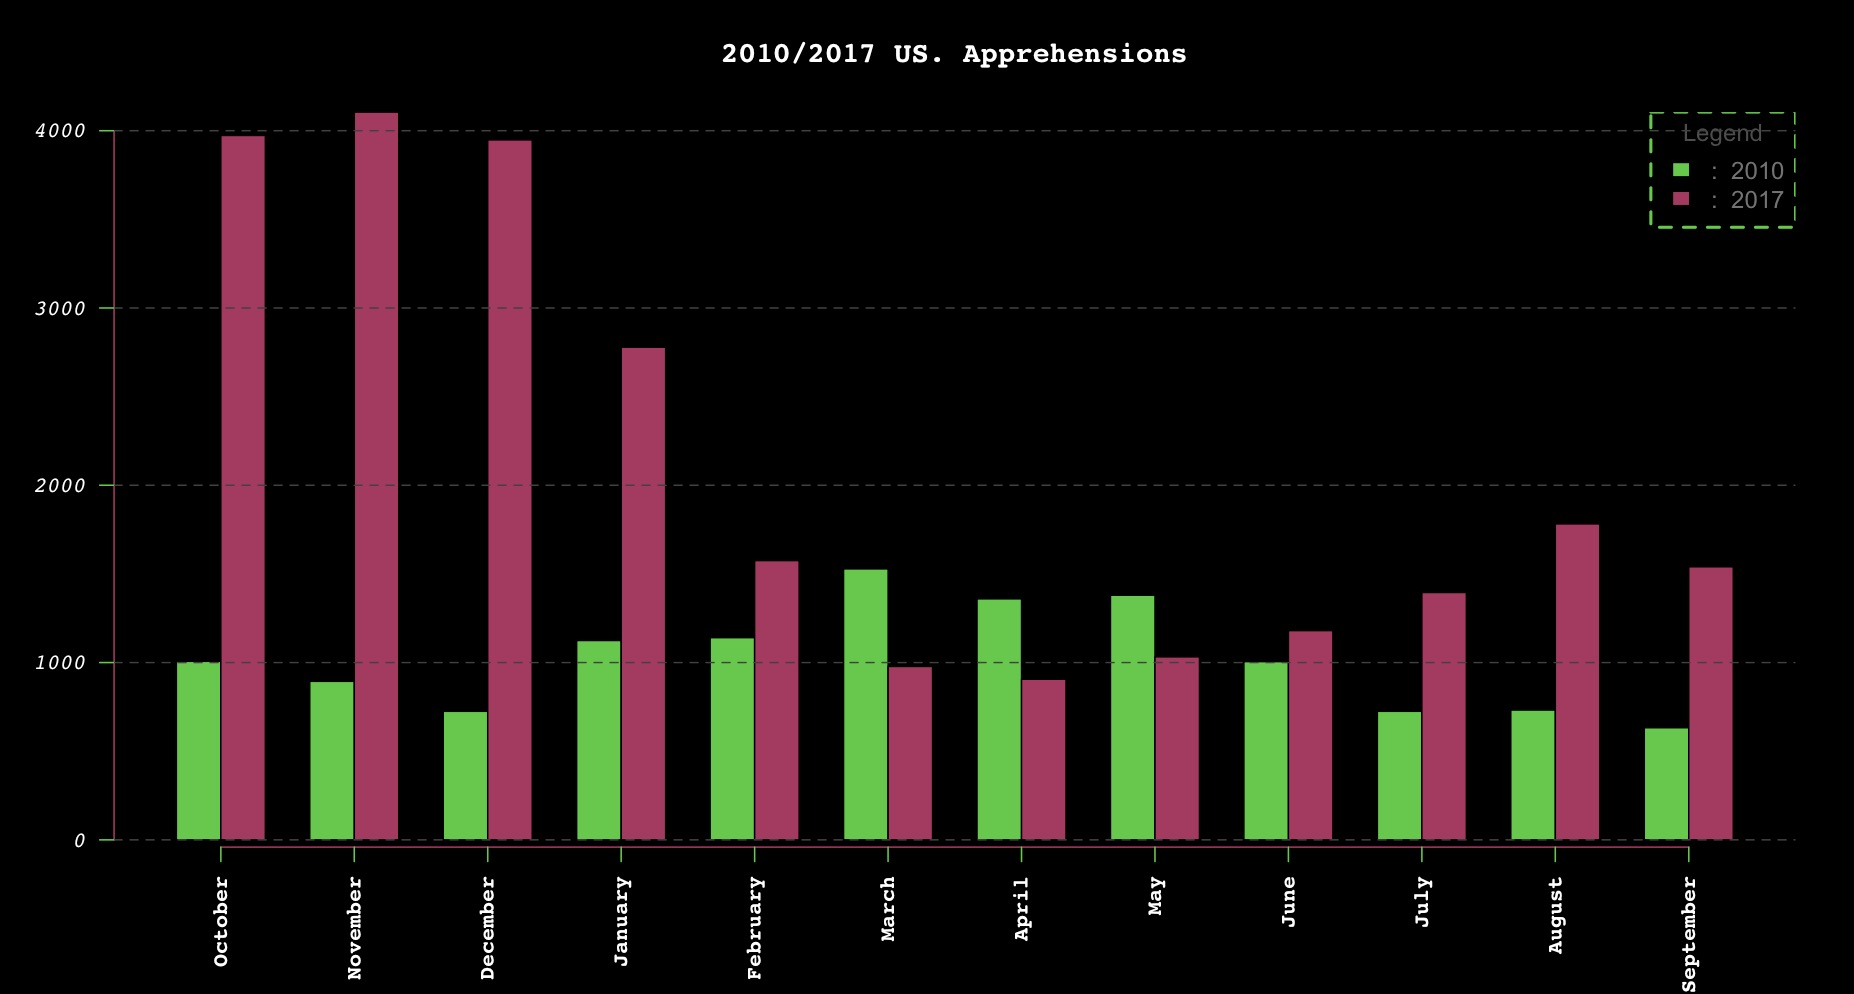
\includegraphics[ height=8cm, width=16cm]{RioGrandeValley}
\caption{Sector: Rio Grande Valley Apprehensions Plot}
\end{figure}
.\\

\begin{figure}[h]
\centering
\includegraphics[ height=4cm, width=11cm]{RioGrandepic}
\caption{Rio Grande Valley}
\end{figure}

\begin{figure}[h]
\centering
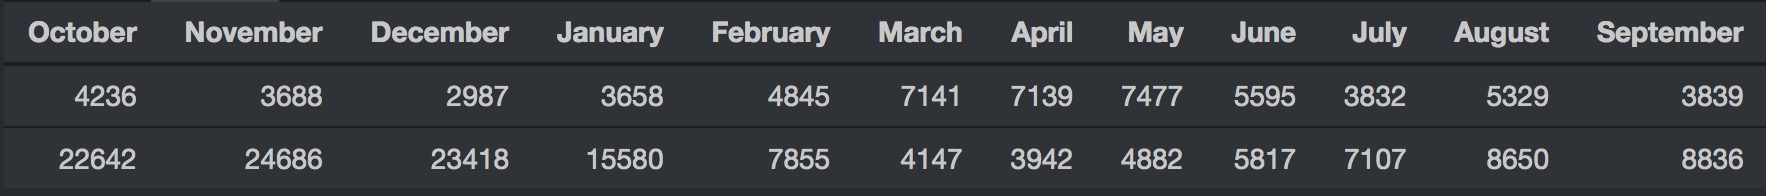
\includegraphics{RioGrandeValleyTable}
\caption{Sector: Rio Grande Valley Apprehensions Table}
\end{figure}

\pagebreak

\subsection{SanDiego}

\begin{figure}[h]
\centering
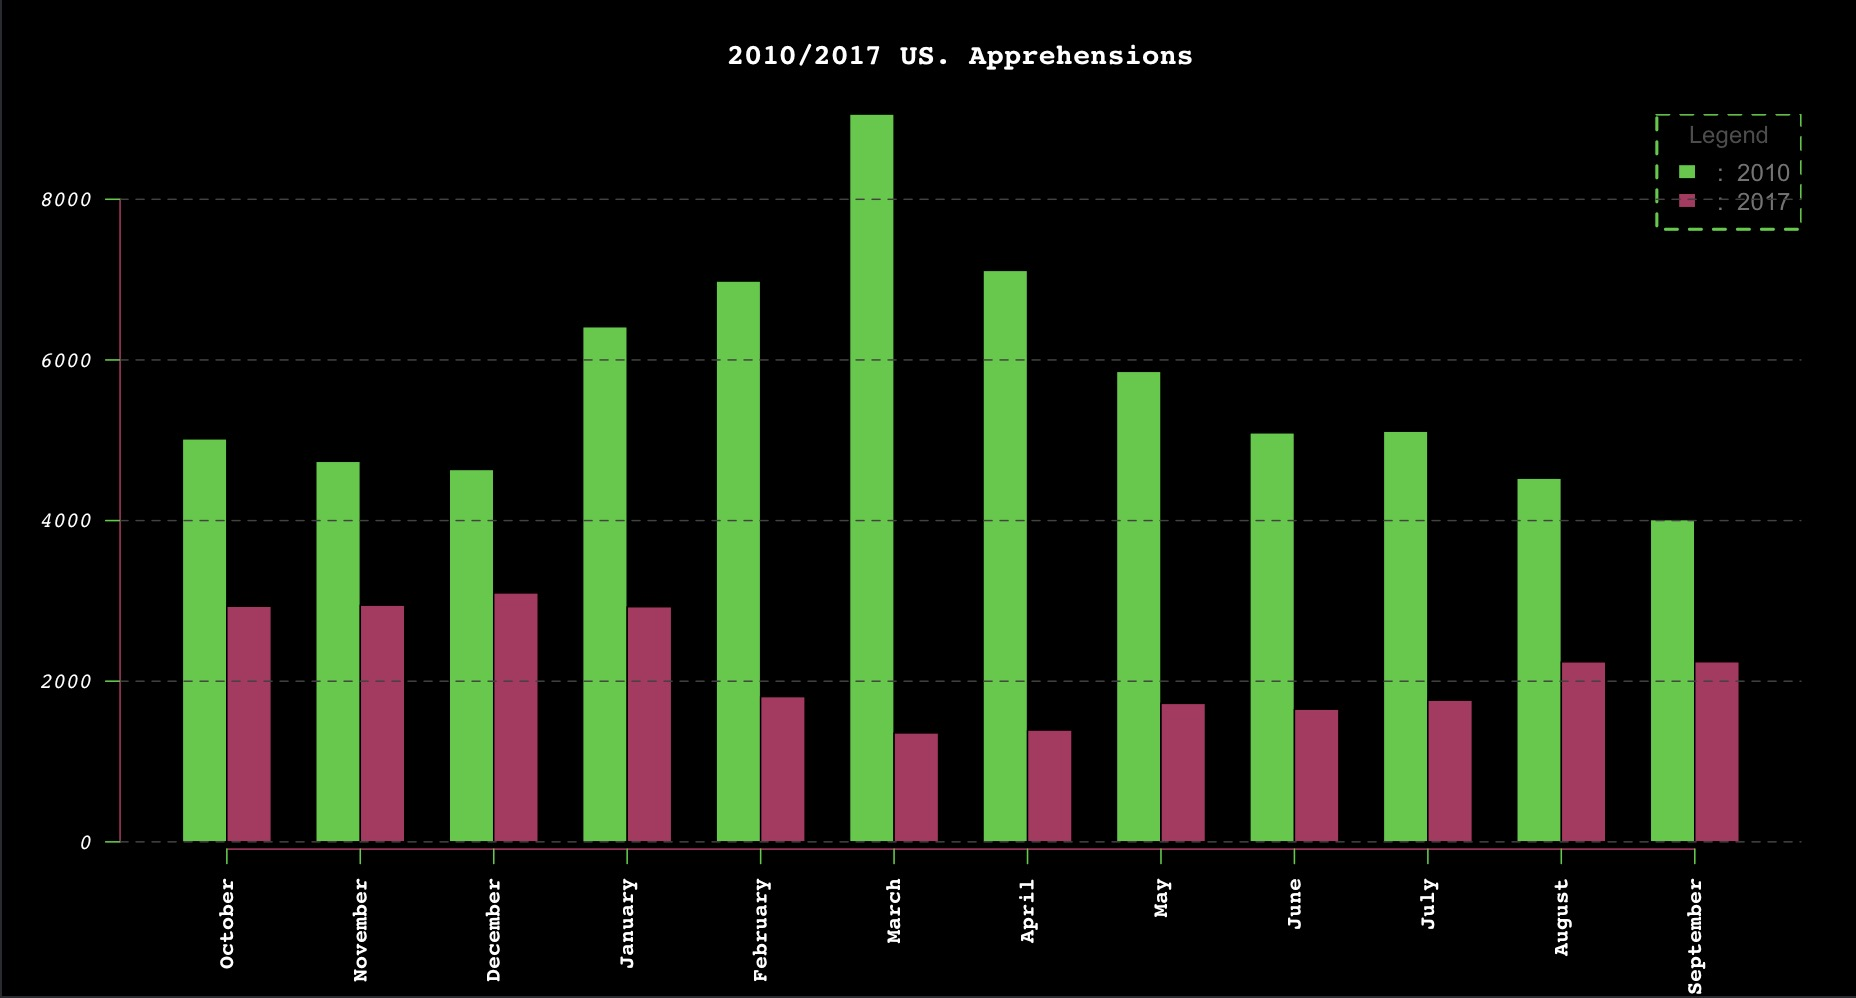
\includegraphics[ height=8cm, width=16cm]{SanDiego}
\caption{Sector: SanDiego Apprehensions Plot}
\end{figure}
.\\

\begin{figure}[h]
\centering
\includegraphics[ height=4cm, width=11cm]{SanDiegopic}
\caption{SanDiego}
\end{figure}

\begin{figure}[h]
\centering
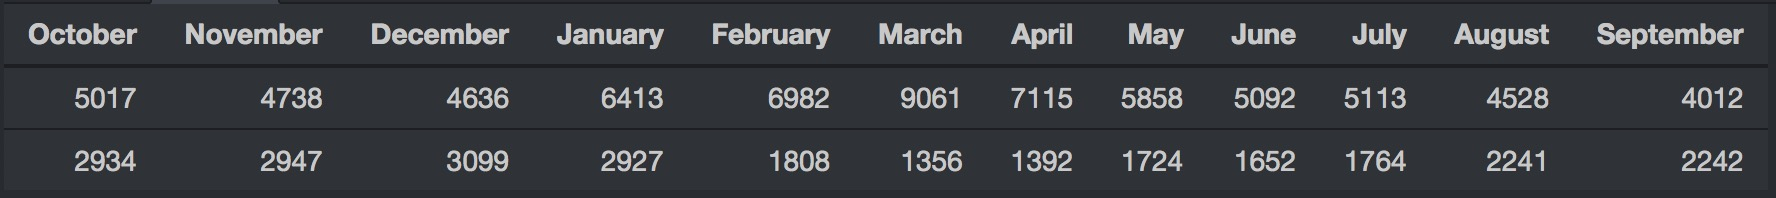
\includegraphics{SanDiegoTable}
\caption{Sector: SanDiego Apprehensions Table}
\end{figure}

\pagebreak

\subsection{Tucson}

\begin{figure}[h]
\centering
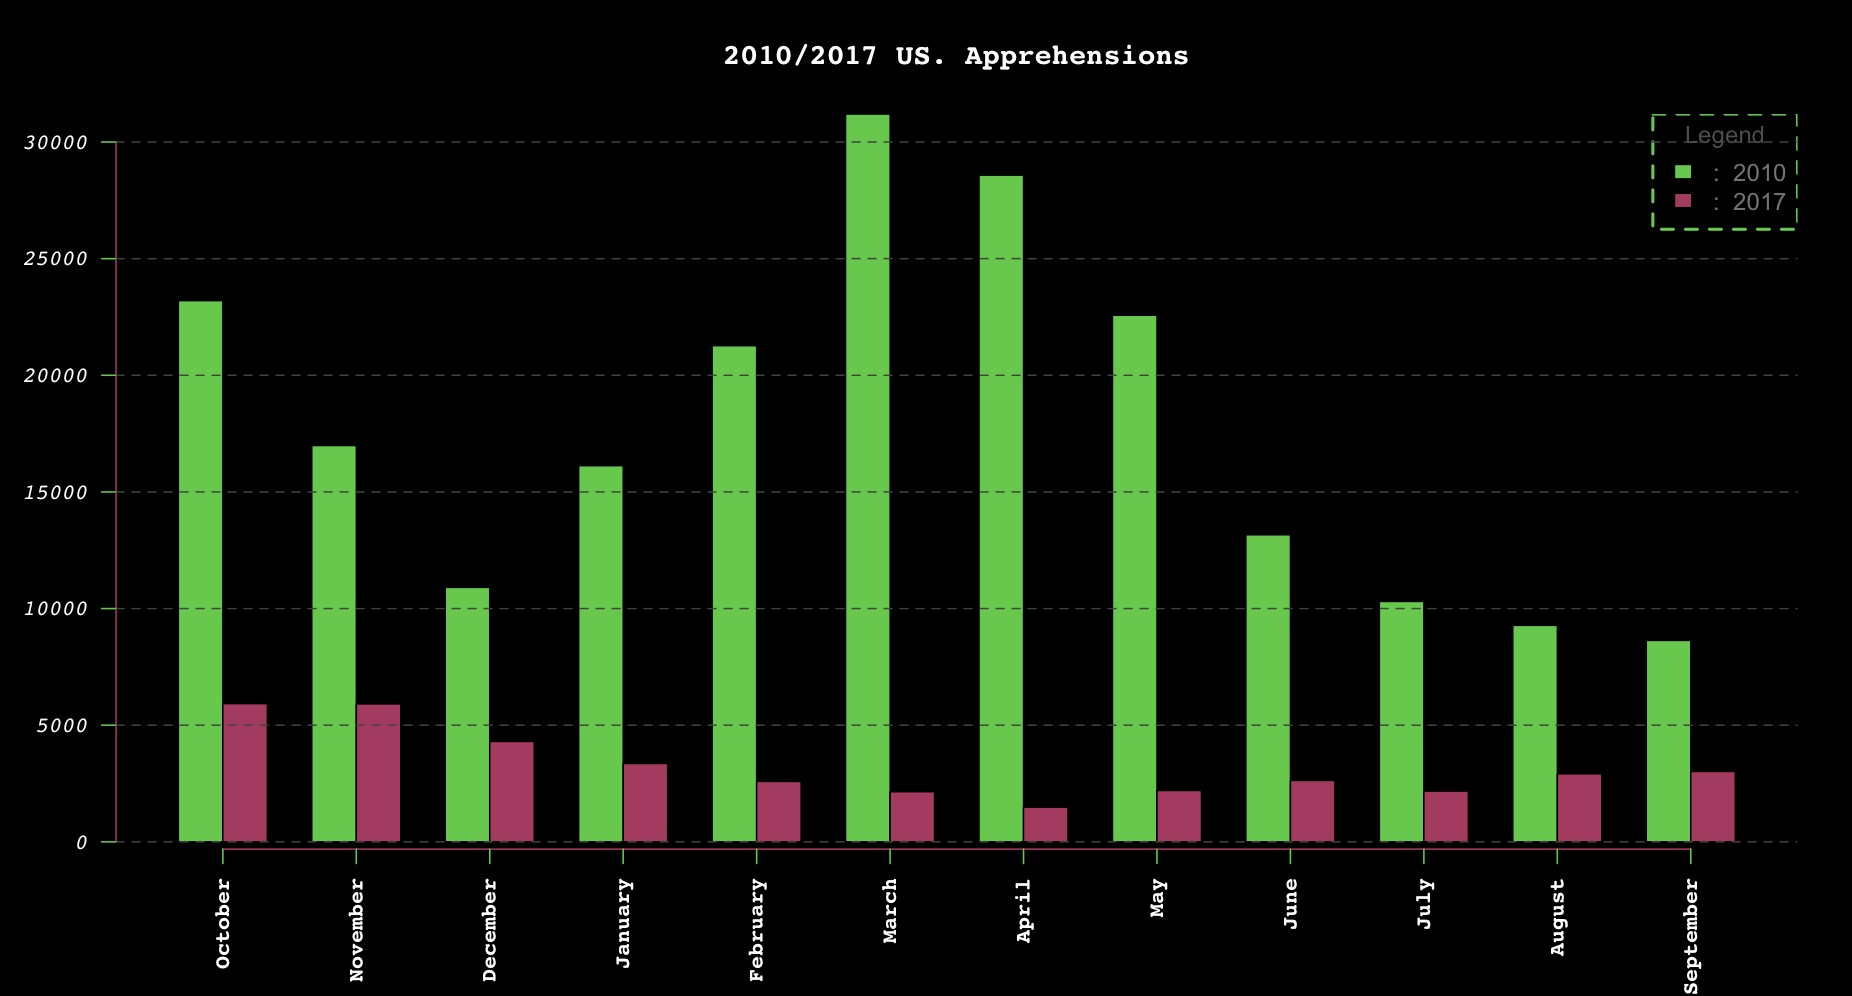
\includegraphics[ height=8cm, width=16cm]{Tucson}
\caption{Sector: Tucson Apprehensions Plot}
\end{figure}
.\\

\begin{figure}[h]
\centering
\includegraphics[ height=4cm, width=11cm]{Tucsonpic}
\caption{Tucson}
\end{figure}

\begin{figure}[h]
\centering
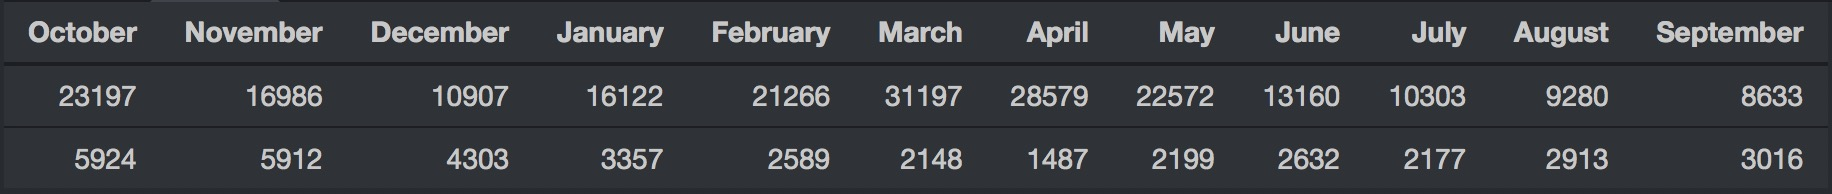
\includegraphics{TucsonTable}
\caption{Sector: Tucson Apprehensions Table}
\end{figure}

\pagebreak

\subsection{Yuma}

\begin{figure}[h]
\centering
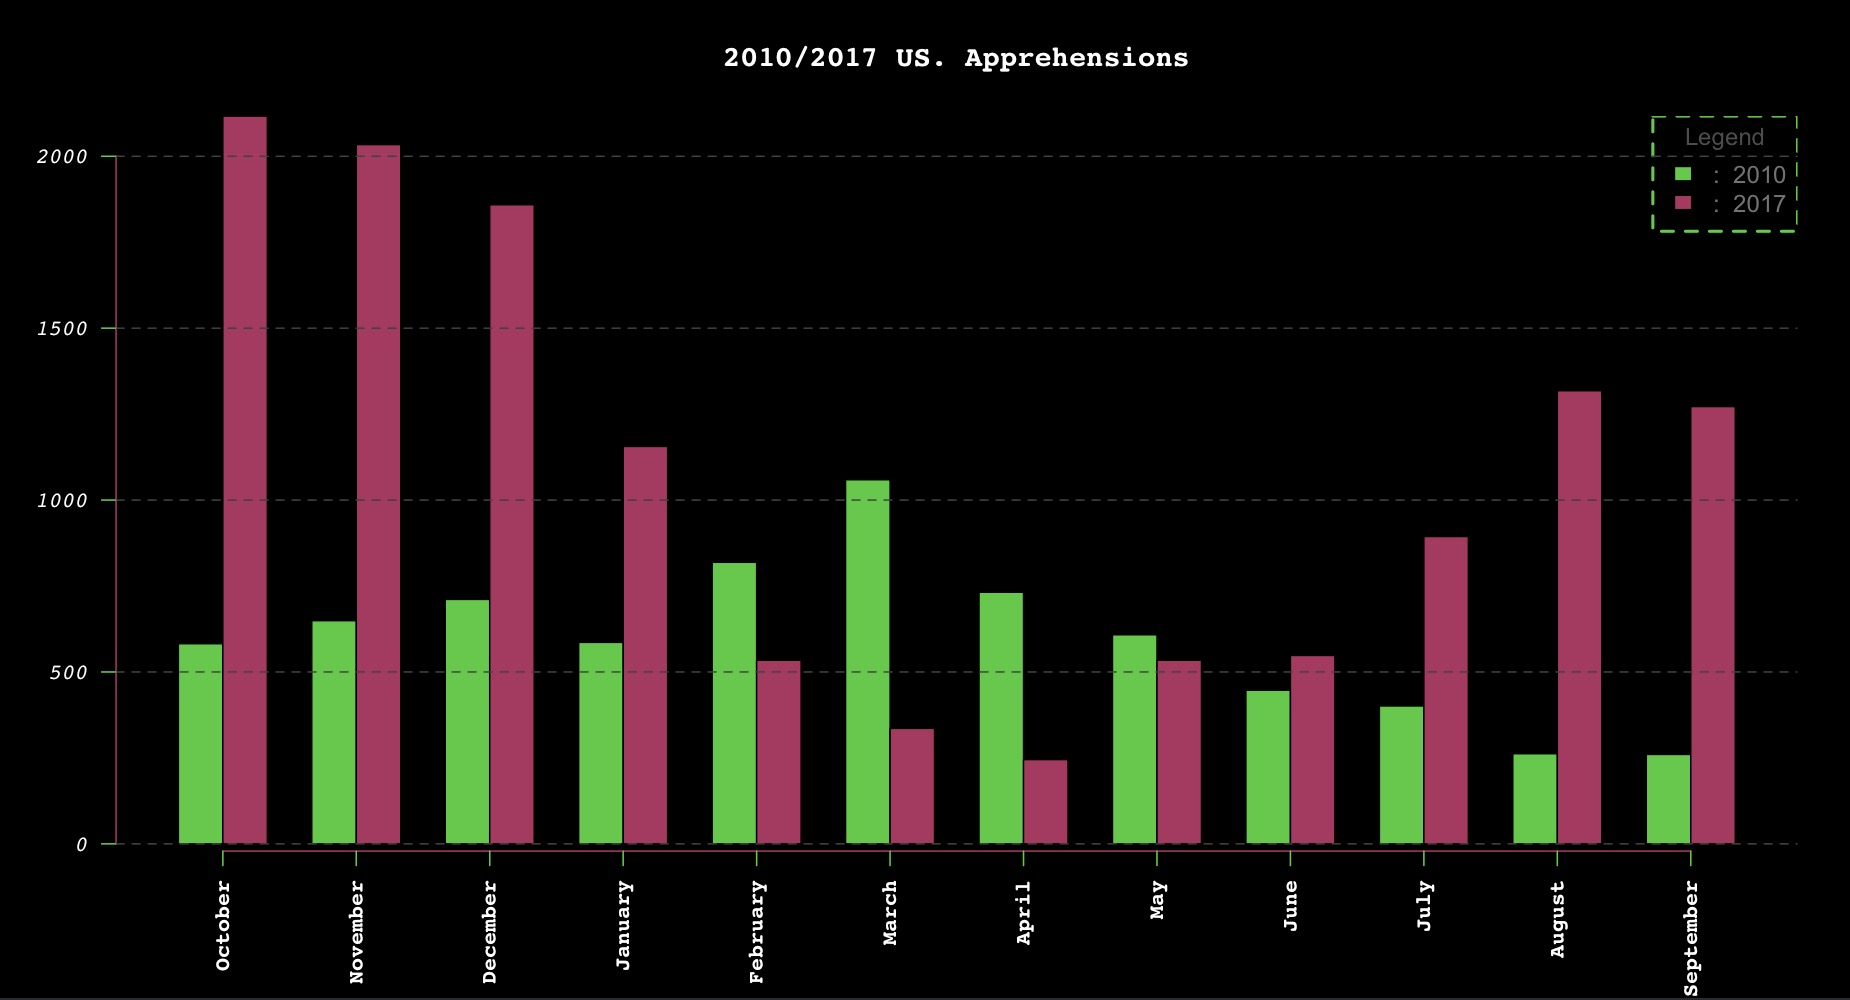
\includegraphics[ height=8cm, width=16cm]{Yuma}
\caption{Sector: Yuma Apprehensions Plot}
\end{figure}
.\\

\begin{figure}[h]
\centering
\includegraphics[ height=4cm, width=11cm]{Yumapic}
\caption{Yuma}
\end{figure}

\begin{figure}[h]
\centering
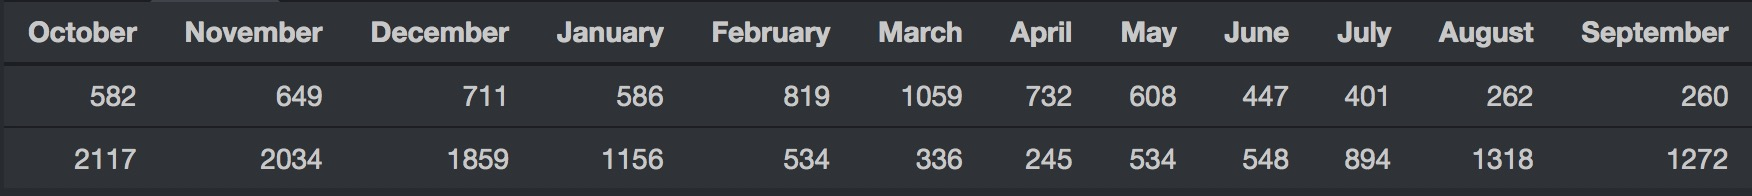
\includegraphics{YumaTable}
\caption{Sector: Yuma Apprehensions Table}
\end{figure}

\pagebreak

\subsection{Statistical Tests}
\begin{center}
Below are some statistical tests on the 2010 and 2017 data.\\
.\\

\end{center}
\begin{Schunk}
\begin{Sinput}
> data2010 <- read.csv('BP Apprehensions 2010.csv')
> data2017 <- read.csv('PB Apprehensions 2017.csv')
> a10.data = data2010$April
> a17.data = data2017$April
> t.test(a10.data, a17.data, paired = TRUE)
\end{Sinput}
\begin{Soutput}
	Paired t-test

data:  a10.data and a17.data
t = 1.7273, df = 8, p-value = 0.1224
alternative hypothesis: true difference in means is not equal to 0
95 percent confidence interval:
 -1642.025 11444.247
sample estimates:
mean of the differences 
               4901.111 
\end{Soutput}
\begin{Sinput}
> var.test(a10.data, a17.data)
\end{Sinput}
\begin{Soutput}
	F test to compare two variances

data:  a10.data and a17.data
F = 63.321, num df = 8, denom df = 8, p-value = 3.939e-06
alternative hypothesis: true ratio of variances is not equal to 1
95 percent confidence interval:
  14.28314 280.71787
sample estimates:
ratio of variances 
          63.32087 
\end{Soutput}
\begin{Sinput}
> data2010$Sector= NULL
> summary(data2010)
\end{Sinput}
\begin{Soutput}
    October         November        December        January     
 Min.   :  530   Min.   :  421   Min.   :  373   Min.   :  433  
 1st Qu.: 1007   1st Qu.:  894   1st Qu.:  711   1st Qu.: 1124  
 Median : 2589   Median : 2130   Median : 1802   Median : 2526  
 Mean   : 4543   Mean   : 3646   Mean   : 2782   Mean   : 3865  
 3rd Qu.: 4236   3rd Qu.: 3688   3rd Qu.: 2987   3rd Qu.: 3658  
 Max.   :23197   Max.   :16986   Max.   :10907   Max.   :16122  
    February         March           April            May       
 Min.   :  484   Min.   :  660   Min.   :  575   Min.   :  493  
 1st Qu.: 1140   1st Qu.: 1528   1st Qu.: 1359   1st Qu.: 1380  
 Median : 2836   Median : 4408   Median : 3419   Median : 3126  
 Mean   : 4754   Mean   : 6818   Mean   : 6137   Mean   : 5227  
 3rd Qu.: 4845   3rd Qu.: 7141   3rd Qu.: 7115   3rd Qu.: 5858  
 Max.   :21266   Max.   :31197   Max.   :28579   Max.   :22572  
      June            July           August       September   
 Min.   :  415   Min.   :  280   Min.   : 262   Min.   : 260  
 1st Qu.: 1005   1st Qu.:  725   1st Qu.: 732   1st Qu.: 632  
 Median : 2440   Median : 1857   Median :2075   Median :2042  
 Mean   : 3662   Mean   : 2845   Mean   :2935   Mean   :2533  
 3rd Qu.: 5092   3rd Qu.: 3832   3rd Qu.:4528   3rd Qu.:3839  
 Max.   :13160   Max.   :10303   Max.   :9280   Max.   :8633  
\end{Soutput}
\begin{Sinput}
> data2017$Sector= NULL
> summary(data2017)
\end{Sinput}
\begin{Soutput}
    October         November        December        January         February   
 Min.   :  697   Min.   :  603   Min.   :  477   Min.   :  473   Min.   : 383  
 1st Qu.: 2117   1st Qu.: 1880   1st Qu.: 1859   1st Qu.: 1243   1st Qu.:1104  
 Median : 2934   Median : 2947   Median : 2460   Median : 2265   Median :1575  
 Mean   : 5132   Mean   : 5246   Mean   : 4806   Mean   : 3508   Mean   :2084  
 3rd Qu.: 3973   3rd Qu.: 4105   3rd Qu.: 3948   3rd Qu.: 2927   3rd Qu.:1808  
 Max.   :22642   Max.   :24686   Max.   :23418   Max.   :15580   Max.   :7855  
     March          April           May            June           July     
 Min.   : 336   Min.   : 245   Min.   : 534   Min.   : 378   Min.   : 492  
 1st Qu.: 746   1st Qu.: 589   1st Qu.: 740   1st Qu.: 761   1st Qu.: 894  
 Median : 978   Median : 906   Median :1134   Median :1280   Median :1478  
 Mean   :1355   Mean   :1236   Mean   :1613   Mean   :1787   Mean   :2021  
 3rd Qu.:1356   3rd Qu.:1392   3rd Qu.:1724   3rd Qu.:1839   3rd Qu.:2120  
 Max.   :4147   Max.   :3942   Max.   :4882   Max.   :5817   Max.   :7107  
     August       September   
 Min.   : 563   Min.   : 614  
 1st Qu.:1318   1st Qu.:1272  
 Median :1880   Median :1988  
 Mean   :2476   Mean   :2504  
 3rd Qu.:2241   3rd Qu.:2242  
 Max.   :8650   Max.   :8836  
\end{Soutput}
\end{Schunk}

\end{document}
